\documentclass[../main.tex]{subfiles}

\begin{document}

\chapter{Transcriptomic analysis of plasmodesmatal response to fungal chitin}
\label{cha:transcripts}

\section{Introduction}
It is well established that plasmodesmata react and respond to microbe presence
through the recognition of highly-conserved microbe associated molecular
patterns (MAMPs) by pattern recognition receptors (PRRs)
\cite{zipfelPlantPatternrecognitionReceptors2014a,
  chevalPlasmodesmalRegulationPlant2018}. One specific interaction of a protein
and a ligand which has been identified is between fungal chitin and CHITIN
ELCITOR RECEPTOR KINASE 1 (CERK1) \cite{miyaCERK1LysMReceptor2007}, were it has
been reported that CERK1 acts a receptor specific to chitin signalling (figure
\ref{fig:receptors}). Interestingly, it has been show that CERK1 is not a
requirement for plasmodesmatal closure in response to chitin and that another
protein, LYSIN MOTIF DOMAIN-CONTAINING GLYCOSYLPHOSPHATIDYLINOSITOL-ANCHORED
PROTEIN 2 (LYM2), is essential for a plasmodesmata; defence response to chitin
\cite{Faulkner2013} (Figure \ref{fig:receptors}).

As eluded to by \citet{Faulkner2013} the current literature suggests that there
exists at least two (seemingly) independent signalling pathways involved in
chitin-triggered defence response in plants. Here, we present the outcome and
analysis of data created in collaboration with the Faulkner group which has
provided new insight into the behaviour of the LYM2 and CERK1 pathways in
Arabidopsis.


\begin{figure}[ht]
  \centering
  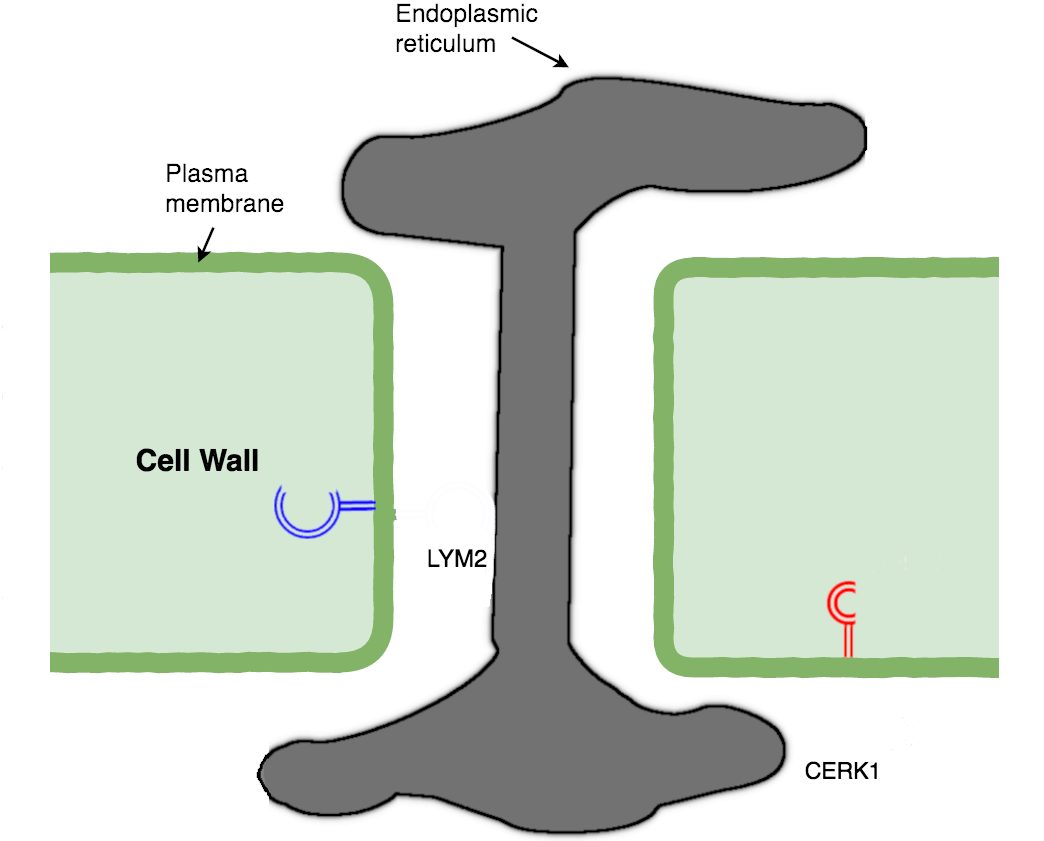
\includegraphics[width=0.5\columnwidth]{figures/original desmotubule.png}
  \caption[Plasmodesmata, \textit{lym2-1} and\textit{cerk2-1}diagram]{\label{fig:receptors}
    An illustrated plasmodesmata channel, with two
    known proteins involved in chitin signalling and plasmodesmata response. Red
    showing the canonical chitin detector CERK1, and in blue LYM2 a
    plasmodesmata localised protein}
\end{figure}

\section{Materials and methods}

\subsection{Plant materials}
An RNA-seq assay was performed on three genotypes of Arabidopsis Thaliana to
test for transcripts unique to chitin perception. Col0 used as a control,
as well as \textit{lym2-1} and \textit{cerk2-1} which are knock-out mutants of
their respective chitin perception proteins. 

All three of these genotypes were grown \textit{in vitro}, as seedlings they
were introduced to one of two treatments. Either chitin or water solutions were
added and mixed into their suspension. Samples were taken at 30 minutes post
treatment and at 6 hours. Whole seedlings were taken and pooled and sequenced
together for robustness. Three replicates of each genotype, treatment and time
point were produced.


\subsection{Computational methods}

Data were pre-processed firstly through removing adaptor sequences, with
\textit{trimmomatic} \cite{bolgerTrimmomaticFlexibleTrimmer2014}. Sanity checks
were performed using \textit{fastqc} \cite{andrewsBabrahamBioinformaticsFastQC}.
Alignment was carried out using a combination of \textit{samtools} and
\textit{hisat2} \cite{liSequenceAlignmentMap2009}. Finally, \textit{htseq-count}
was used to prepare sequence counts from trimmed and aligned RNA-seq data
\cite{kimHISATFastSpliced2015}. Preparation of count data used the method
described by \citet{loveModeratedEstimationFold2014a} and normalised transcript
counts were created using \textit{DESEQ2}
\cite{piperCountNormalizationDESeq22017}.

With these normalised data, we calculated the false discovery rate (FDR) value
for chitin compared to water treatments of each genotype at each time point. We
specified that all genes with an FDR$< 0.05$ would be considered significant.
For further down-stream gene-ontology (GO) analysis we used
\cite{klopfensteinGOATOOLSPythonLibrary2018}, and further limited genes of
interest to having a Log2 Fold Change (LFC) of $>2$ to select only genes with a
high degree of difference from their water treatment.

\section{Analysis of chitin response after 30 minutes}
\label{sec:seqresults}

\subsection{Col0 and \textit{lym2-1} respond strongly to chitin}

Initial analysis indicates that at our earliest time point, 30 minutes post
treatment, a significant response to chitin is seen in both Col0 and
\textit{lym2-1}. Unsurprisingly, \textit{cerk2-1} produced only 3 differentially
expressed genes (DEGs) whereas Col0 and \textit{lym2-1} show to have 3664 and
5196 respectively (Figure \ref{fig:05hrDEGs}). A surprising result is seen in that the
\textit{lym2-1} mutant had a much higher level of mis-regulation following
chitin treatment of $\approx70\%$ more genes classified as significantly different
than the control.

\begin{figure}[ht]
  \centering
  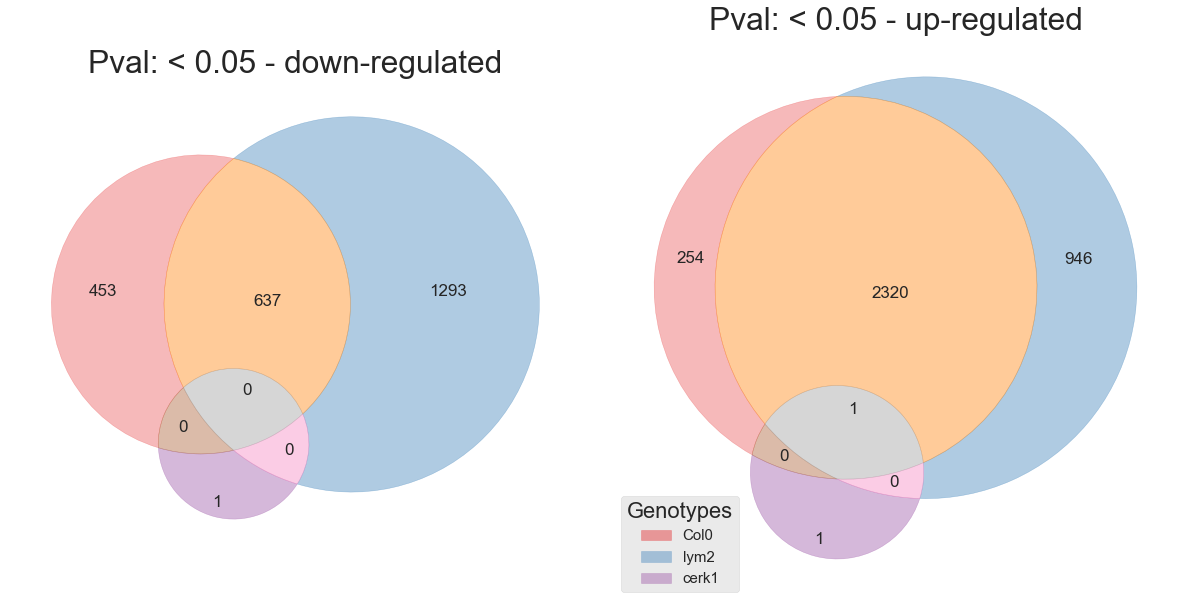
\includegraphics[width=0.6\columnwidth]{figures/vennTreatmentschitin.png}
  \caption{\label{fig:05hrDEGs} Venn diagram of differential genes for Col0,
    \textit{cerk2-1} and \textit{lym2-1} 30 minutes after exposed to chitin}
\end{figure}

\subsection{\textit{cerk2-1} is required for a substantial transcriptional response to chitin}

Comparing the most DEGs for each genotype reveals that a similar expression
profile is seen in up-regulated genes for both Col0 and \textit{lym2-1} , while
\textit{cerk2-1} doesn't show any genes that would be classified as having a
substantially different expression compared with the water control (DEGs with
greater than 2 LFC) (Figure \ref{subfig-1:deg5}). In genes down-regulated at 30
minutes post-treatment, \textit{lym2-1} and Col0 have a slight difference.
Overall at this time point \textit{lym2-1} shows a much higher degree of
mis-regulation (Figure \ref{subfig-2:deg5}). This behaviour may suggest that
missing a key piece of plasmodesmata signalling leads to the inability to
correctly contain and regulate gene expression.

\begin{figure}[!ht]
  \centering
  \subfloat[Most up-regulated genes at 30 minutes post-treatment of chitin.
  \label{subfig-2:deg5}]{%
    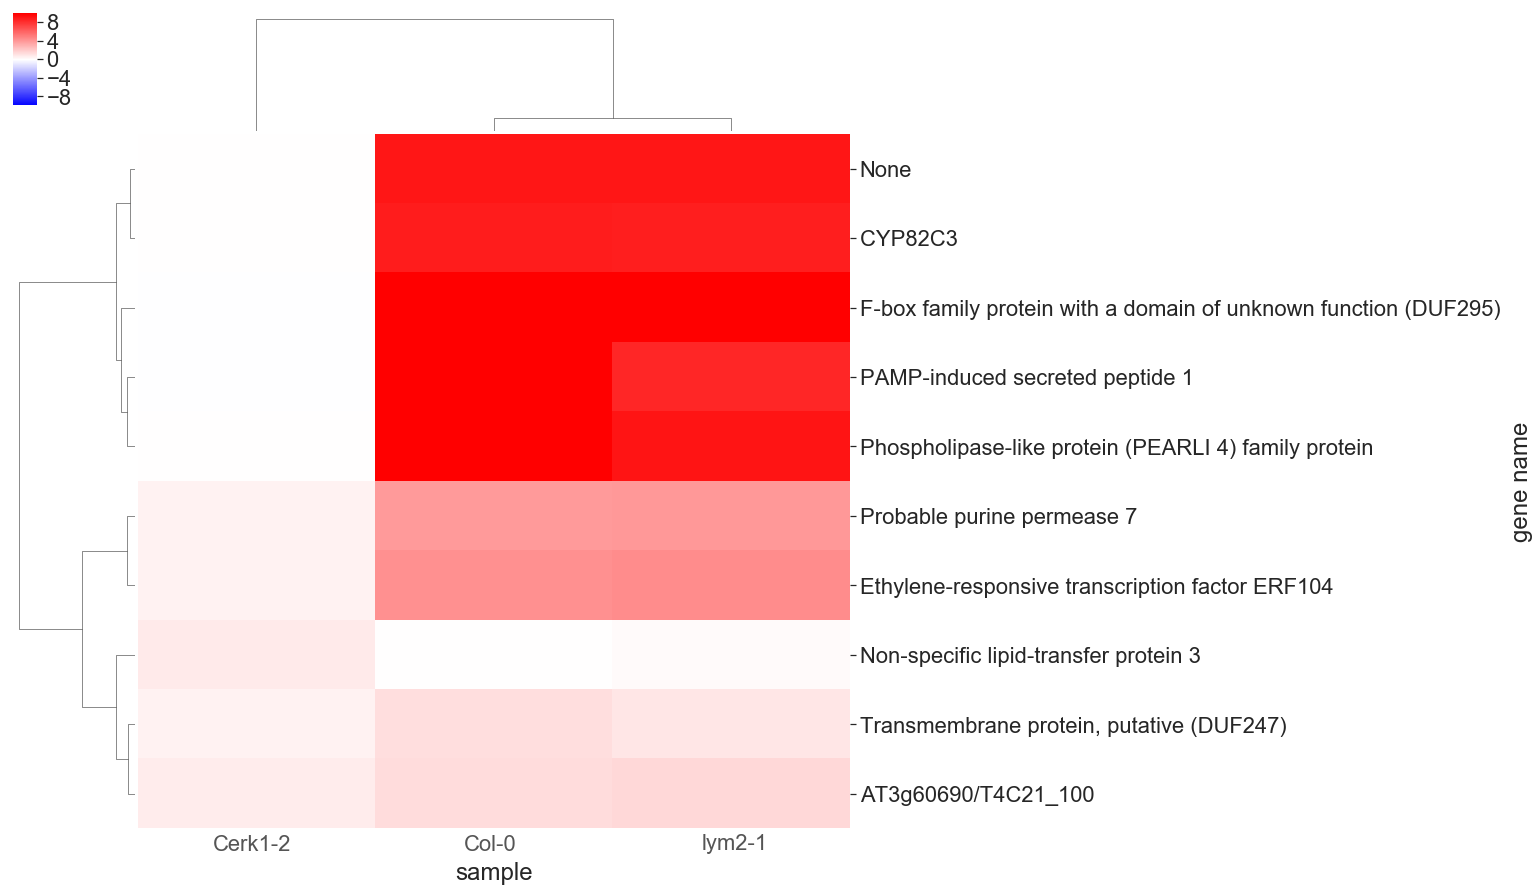
\includegraphics[width=0.7\columnwidth]{./figures/chitin_water_05hr_up.png}
  }
  \\
  \subfloat[Most down-regulated genes at 30 minutes post-treatment of chitin\label{subfig-1:deg5}]{%
    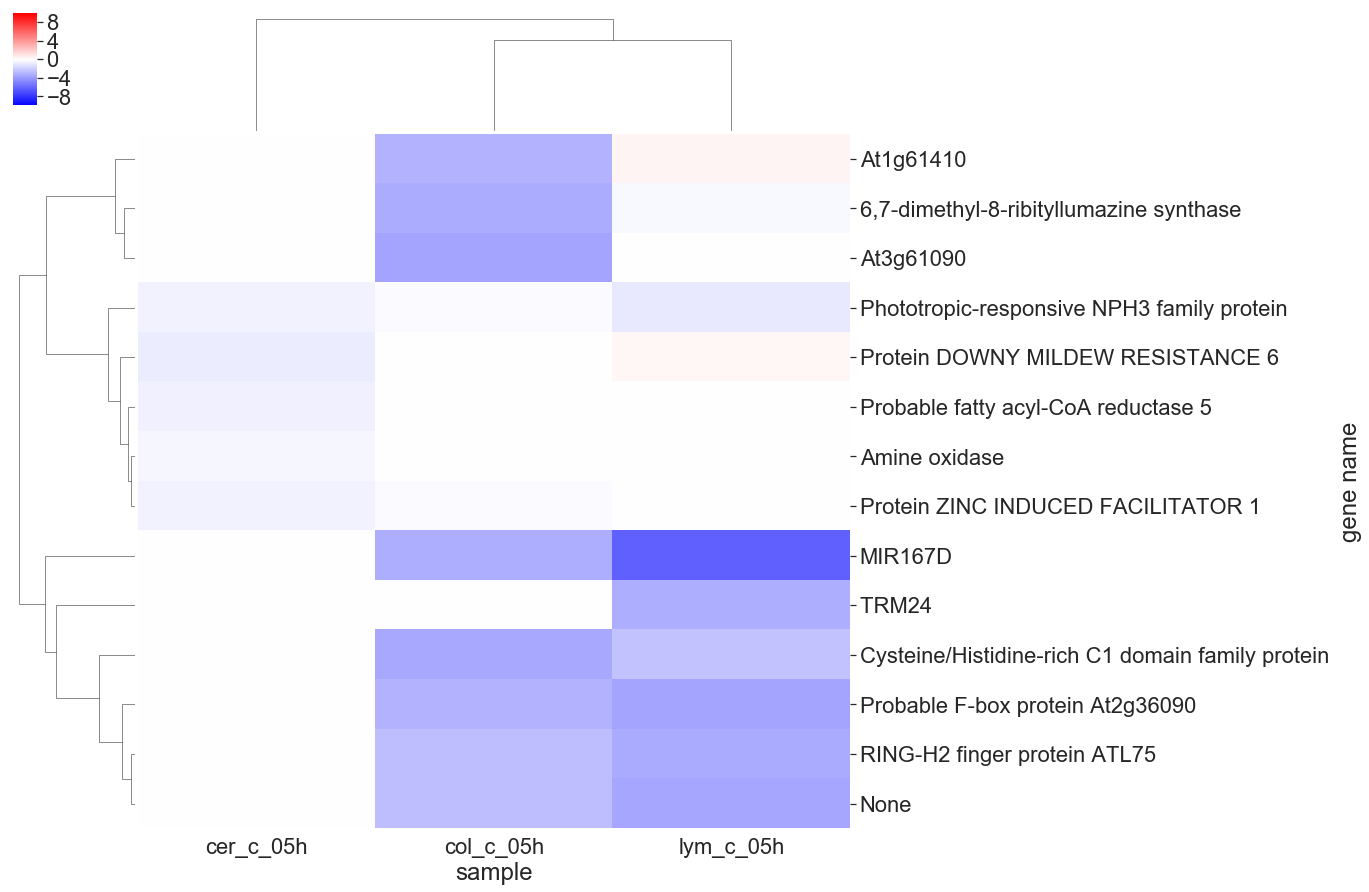
\includegraphics[width=0.7\columnwidth]{./figures/chitin_water_05hr_down.png}
  }
  \caption{5 most up and down regulated genes at 30 minutes post chitin
    treatment for each genotype. Columns show each genotype tested, colour intensity represents LFC}
  \label{fig:DEG5}
\end{figure}


\subsection{\textit{cerk1-2} produces a minor response to chitin}

Of the several thousand DEGs found in this study only three have been shown to
affect \textit{cerk2-1}. AT5G24530 (DMR6) is shown to be uniquely down-regulated when
presented with chitin. Curiously, this gene has previously been described as
enhancing susceptibility to downy mildew \cite{DOWNYMILDEWRESISTANT}, these data
could suggest that a secondary fallback mechanism is activated only when CERK is
not present (Figure \ref{subfig-1:cerk}).

Two other genes that appear to be differentially regulated in \textit{cerk2-1}
AT5G59320 (LTP3) and AT3G60690 (SAUR59) may be worth further consideration. LTP3
has been shown to be involved with abscisic acid, an important signalling
molecule in abiotic stress \cite{vishwakarmaAbscisicAcidSignaling2017} and
SAUR59 is indicated to be a highly mobile transcript
\cite{thiemeEndogenousArabidopsisMessenger2015} and thus potentially involved in
cell-cell communication of stress (Figures \ref{subfig-2:cerk} and
\ref{subfig-3:cerk}).

%  This indicates that chitin perception is not wholly dependant
% on CERK1, as previously thought.  


\begin{figure}[!ht]
  \subfloat[AT5G24530 (DMR6), the single gene found in \textit{cerk1-2} mutants
  which shows a down-regulation in response to chitin \label{subfig-1:cerk}]{%
    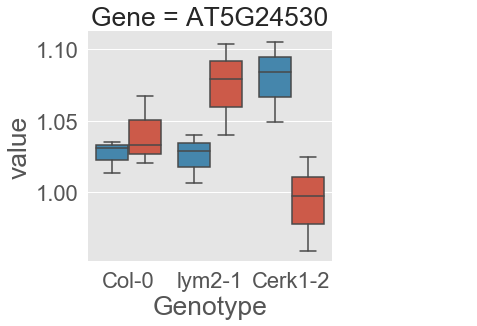
\includegraphics[width=0.5\columnwidth]{./figures/cerk_genes_AT5G24530.png}
  }
  \subfloat[First sub-figure\label{subfig-2:cerk}]{%
    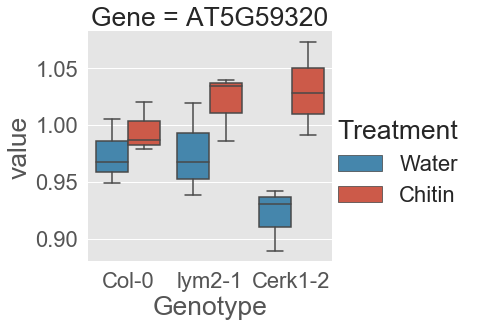
\includegraphics[width=0.5\columnwidth]{./figures/cerk_genes_AT5G59320.png}
  }\\
  \subfloat[First sub-figure\label{subfig-3:cerk}]{%
    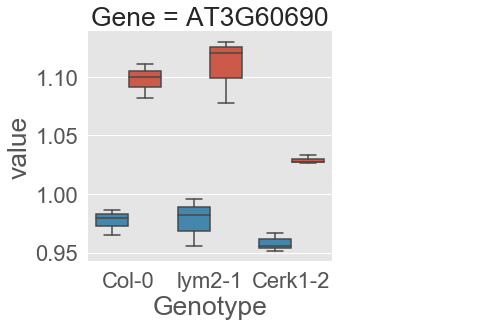
\includegraphics[width=0.5\columnwidth]{./figures/cerk_genes_AT3G60690.png}
  }
  
  \caption{Genes which were found to have a differential regulation in the
    \textit{cerk1-2} genotype. Presented for comparison are the values in both
    Col0 and \textit{lym2-1}, Y values are given as normalised transcript counts
    for each transcript across different treatments (Normalisation was performed
    gene-wise, values are comparative across treatments but not between genes).
    Blue colour in boxplots represents }
  \label{fig:cerk}
\end{figure}

As these data indicate that the effect of knocking-out CERK1 is highly specific,
we hypothesise that CERK1 acts at a high-level and that its absence
inhibits many downstream processes, such as those we see in Col-0 and \textit{lym2-1}.
Our data also maintain and strengthen the established theory that CERK1 and LYM2 are
independent signalling pathways \cite{Faulkner2013, miyaCERK1LysMReceptor2007,
  narusakaPresenceLYM2Dependent2013}.



\subsection{GO term analysis shows Col0 and \textit{lym2-1} have similar
  disruption patterns}


\begin{figure}[ht]
  \centering
  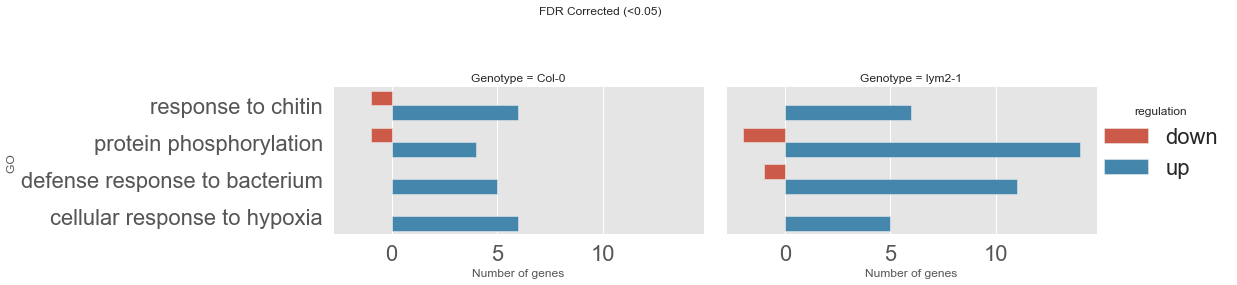
\includegraphics[width=\columnwidth]{figures/05hrGO.png}
  \caption{\label{fig:05hrGO} GO terms for 05hr}
\end{figure}



\begin{figure}[ht]
  \centering
  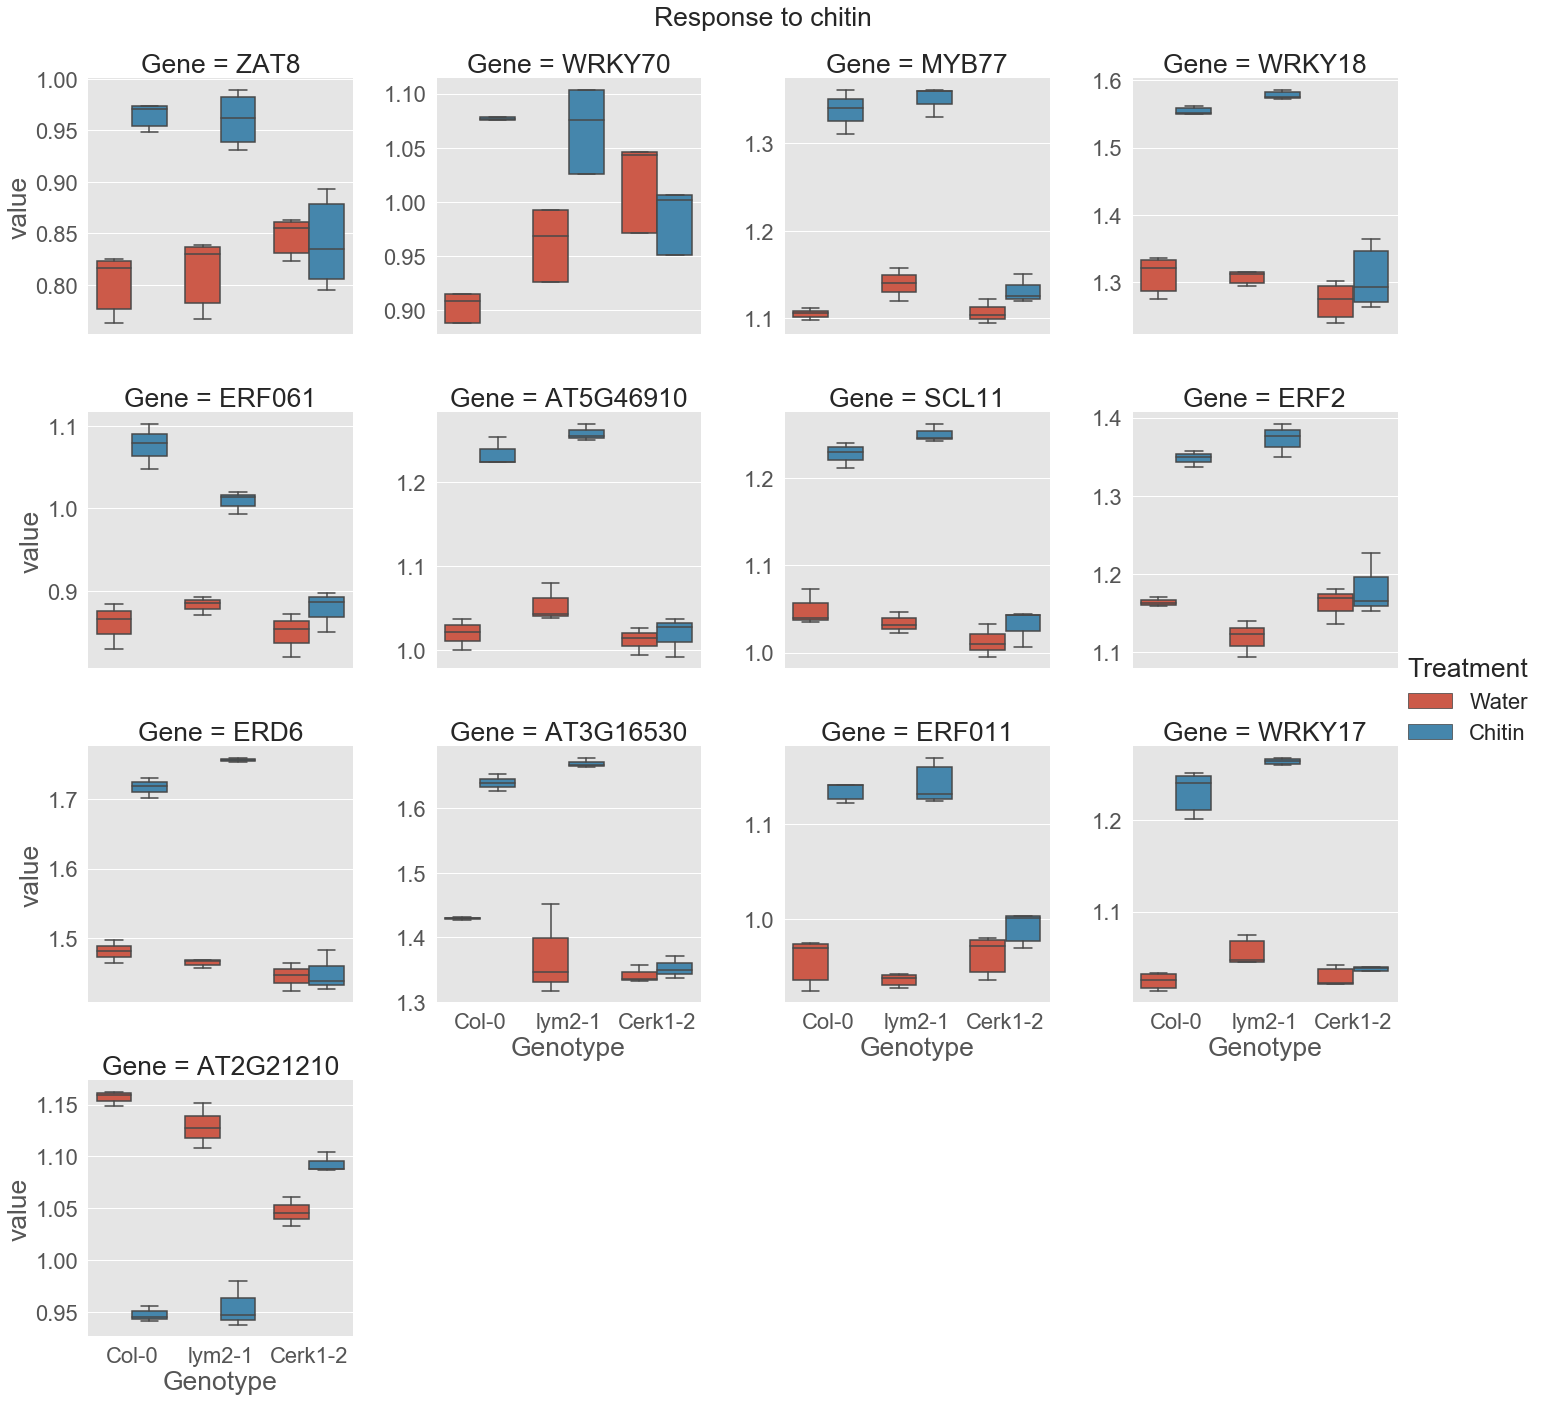
\includegraphics[width=\textwidth, height=\textheight, keepaspectratio]{figures/response to chitin.png}
  \caption{\label{fig:respchitin} Response to chitin genes}
\end{figure}







\section{Temporal gene expression}
\label{sec:tempexpress}



\begin{figure}[!ht]
  \centering
  \subfloat[First sub-figure\label{subfig-1:tmpHist}]{%
    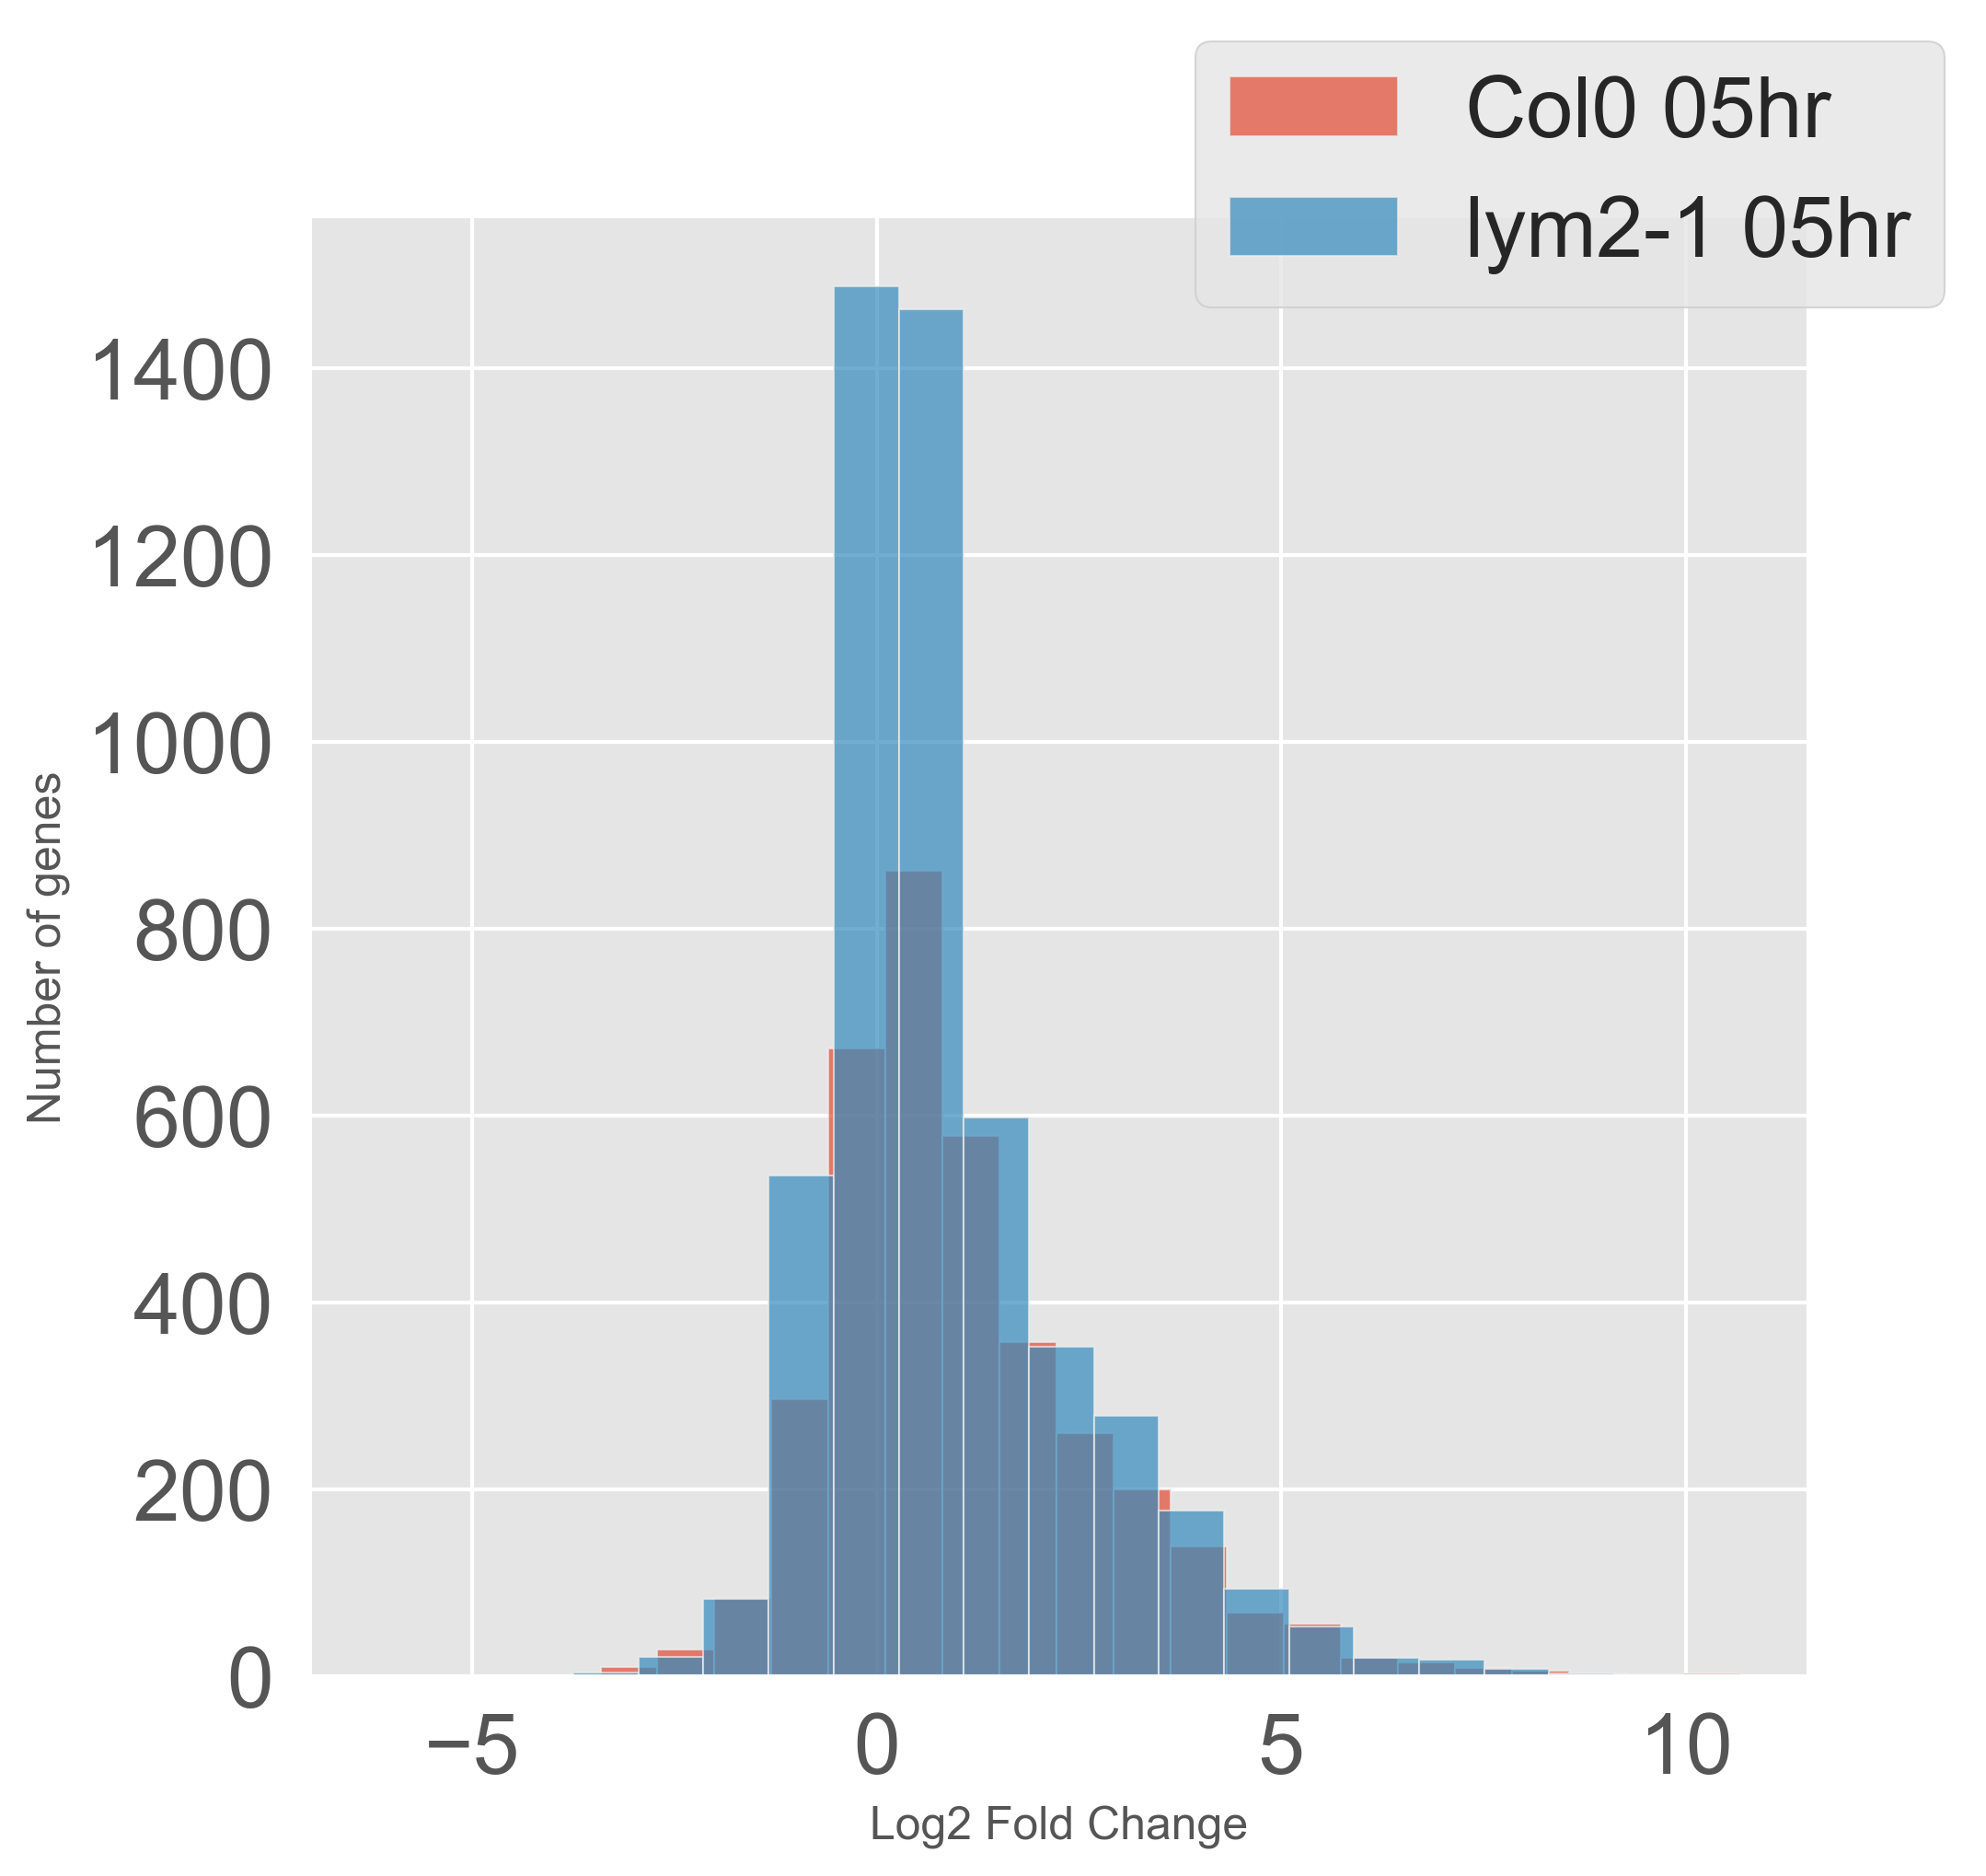
\includegraphics[width=0.3\columnwidth]{./figures/hist05hr.png}
  }
  \subfloat[First sub-figure\label{subfig-2:tmpHist}]{%
    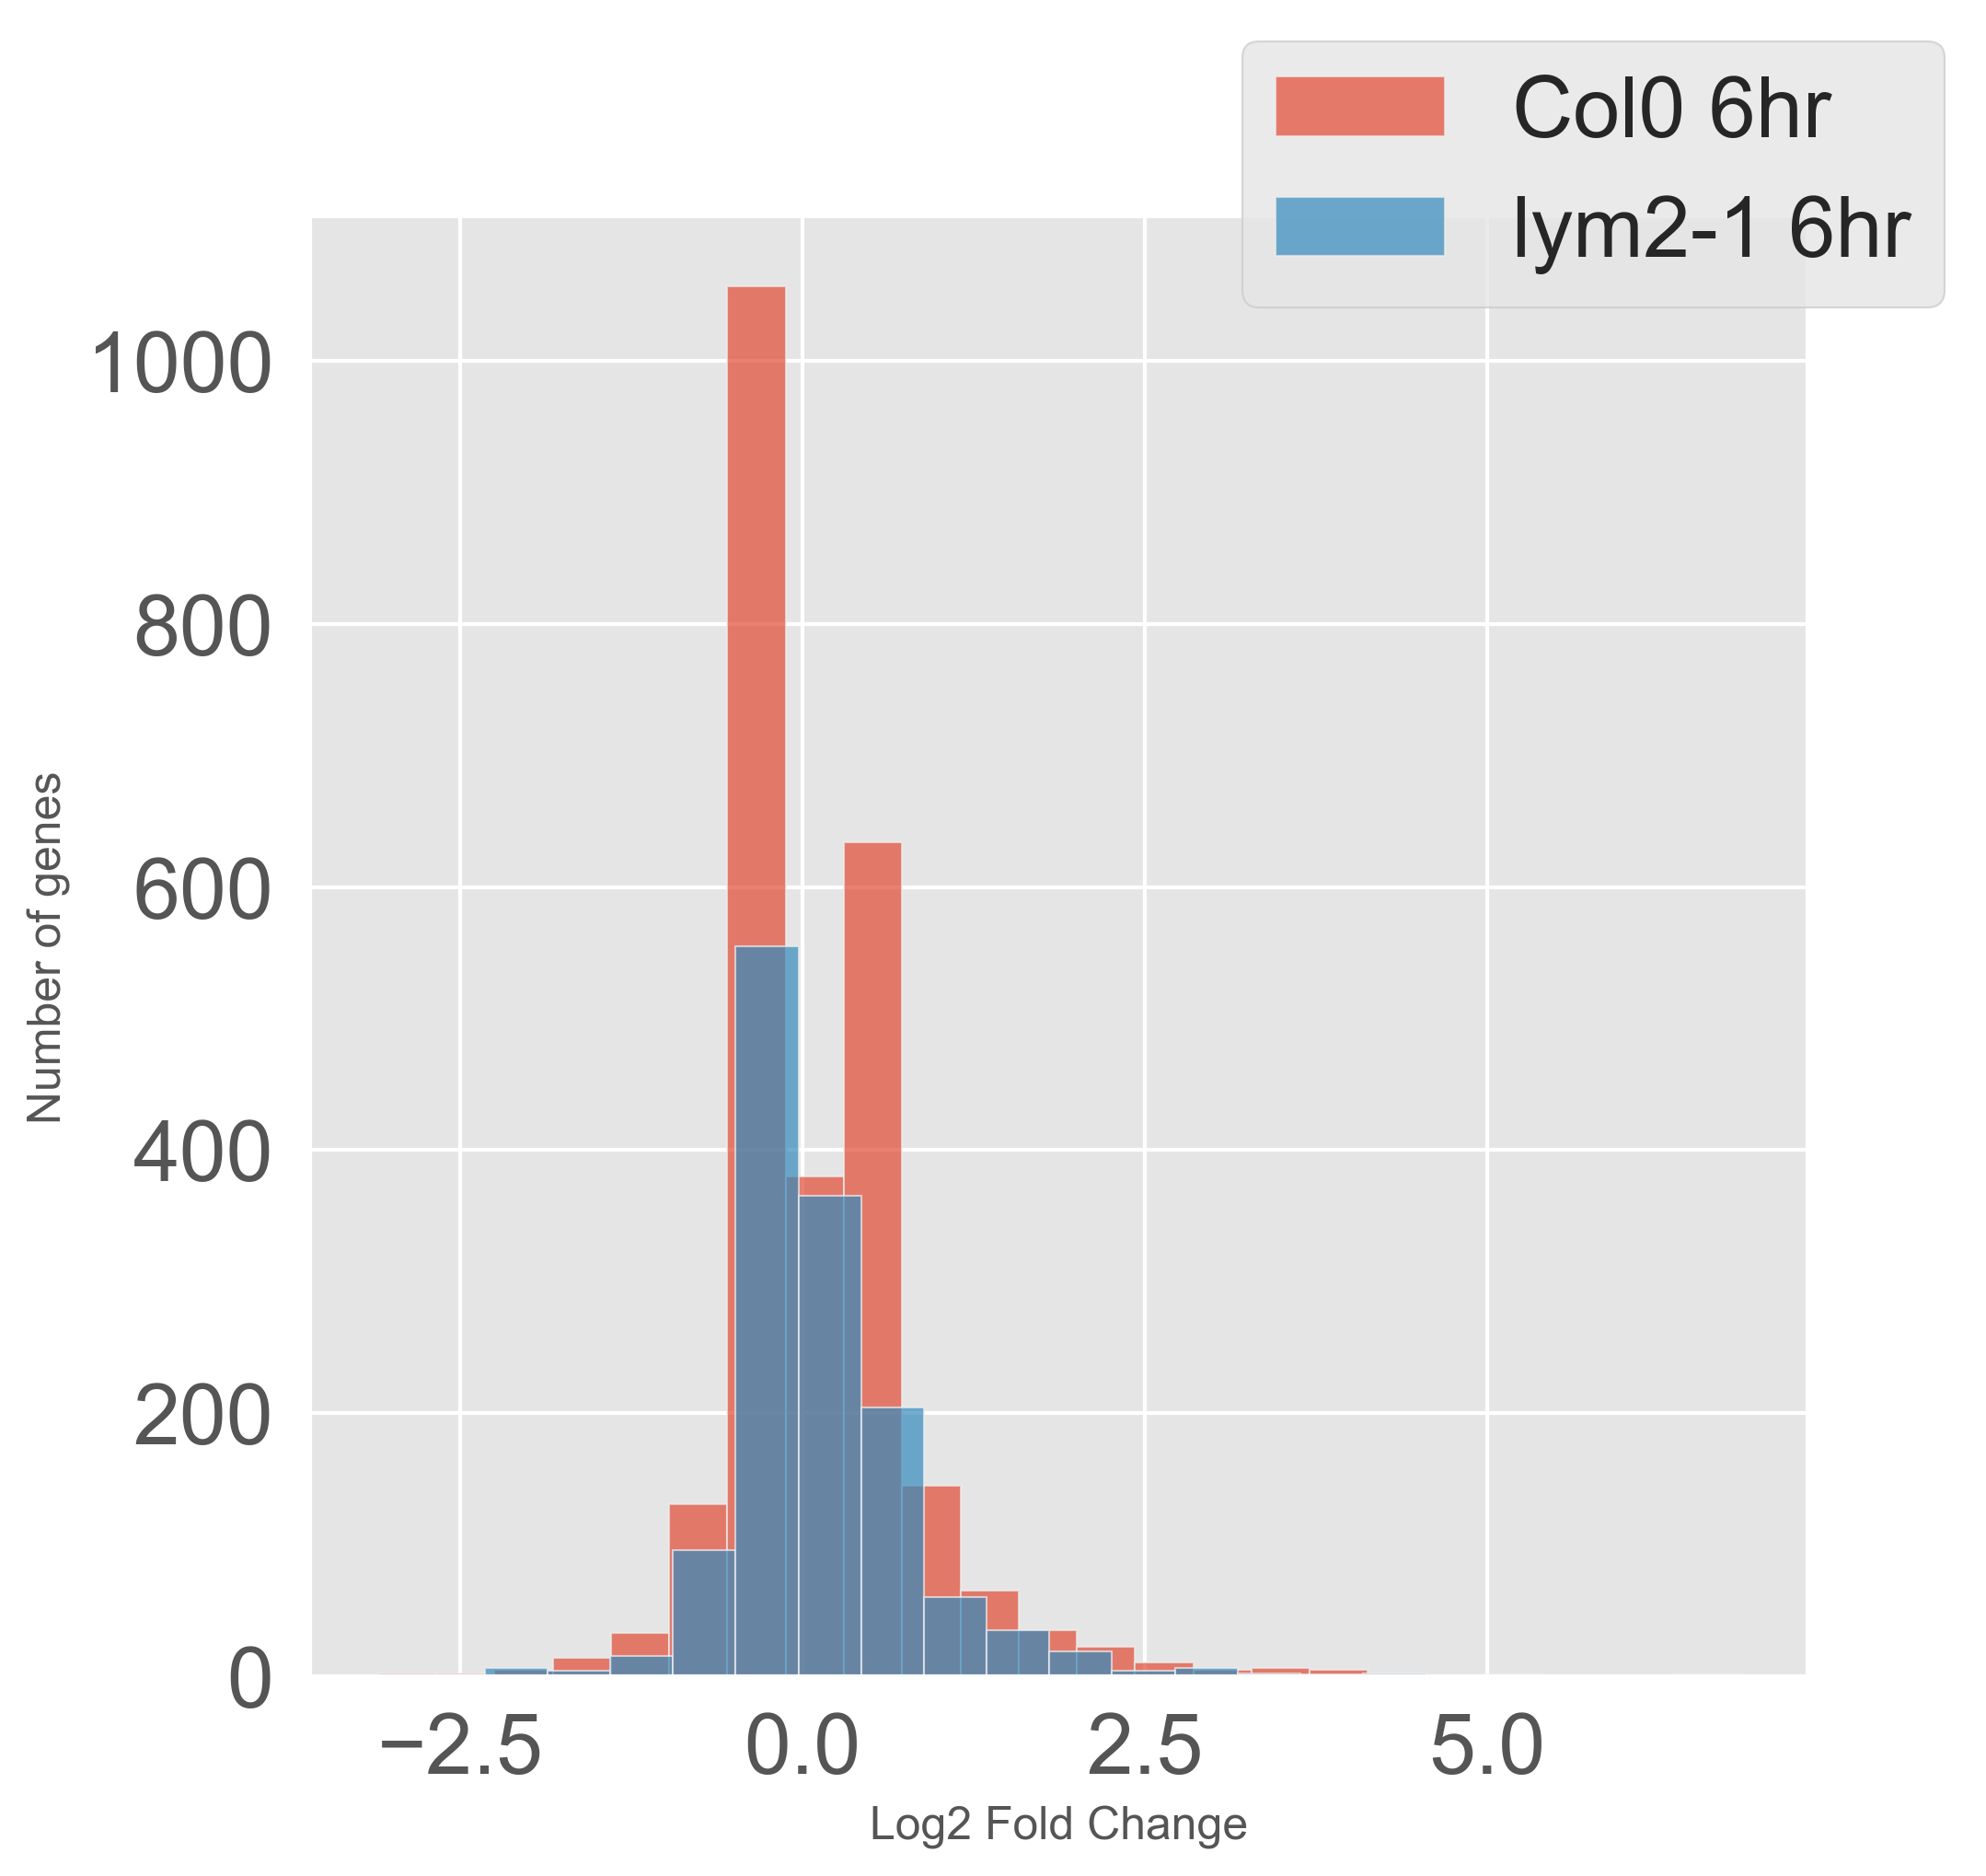
\includegraphics[width=0.3\columnwidth]{./figures/hist_6hr.png}
  }
  \caption{Temporal histograms}
  \label{fig:tmpHist}
\end{figure}



\begin{figure}[!ht]
  \centering
  \subfloat[First sub-figure\label{subfig-1:diverg}]{%
    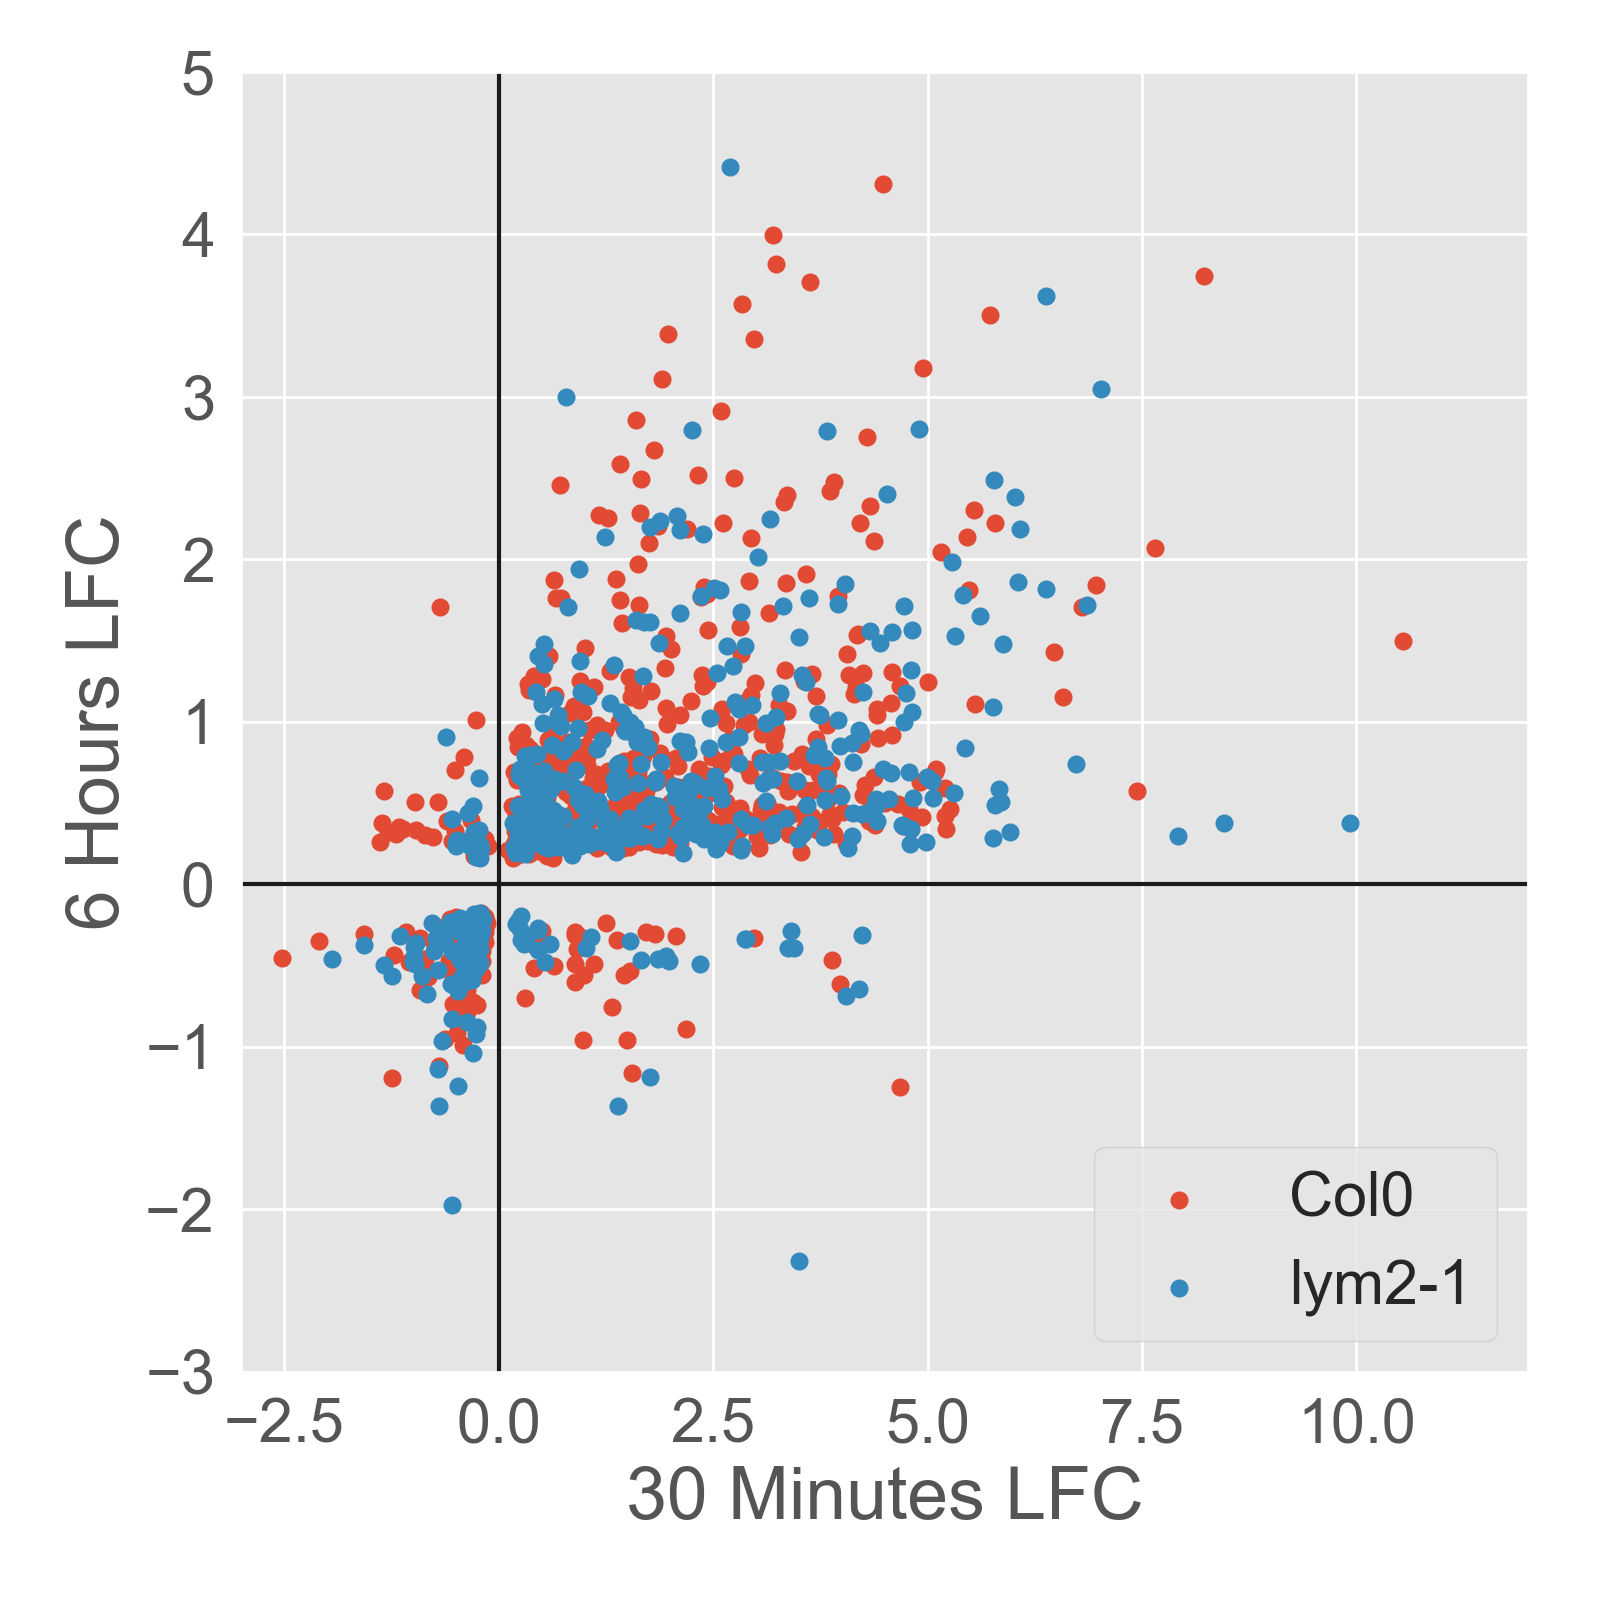
\includegraphics[width=0.5\columnwidth]{./figures/divergingGenes_all.png}
  }
  \subfloat[First sub-figure\label{subfig-2:diverg}]{%
    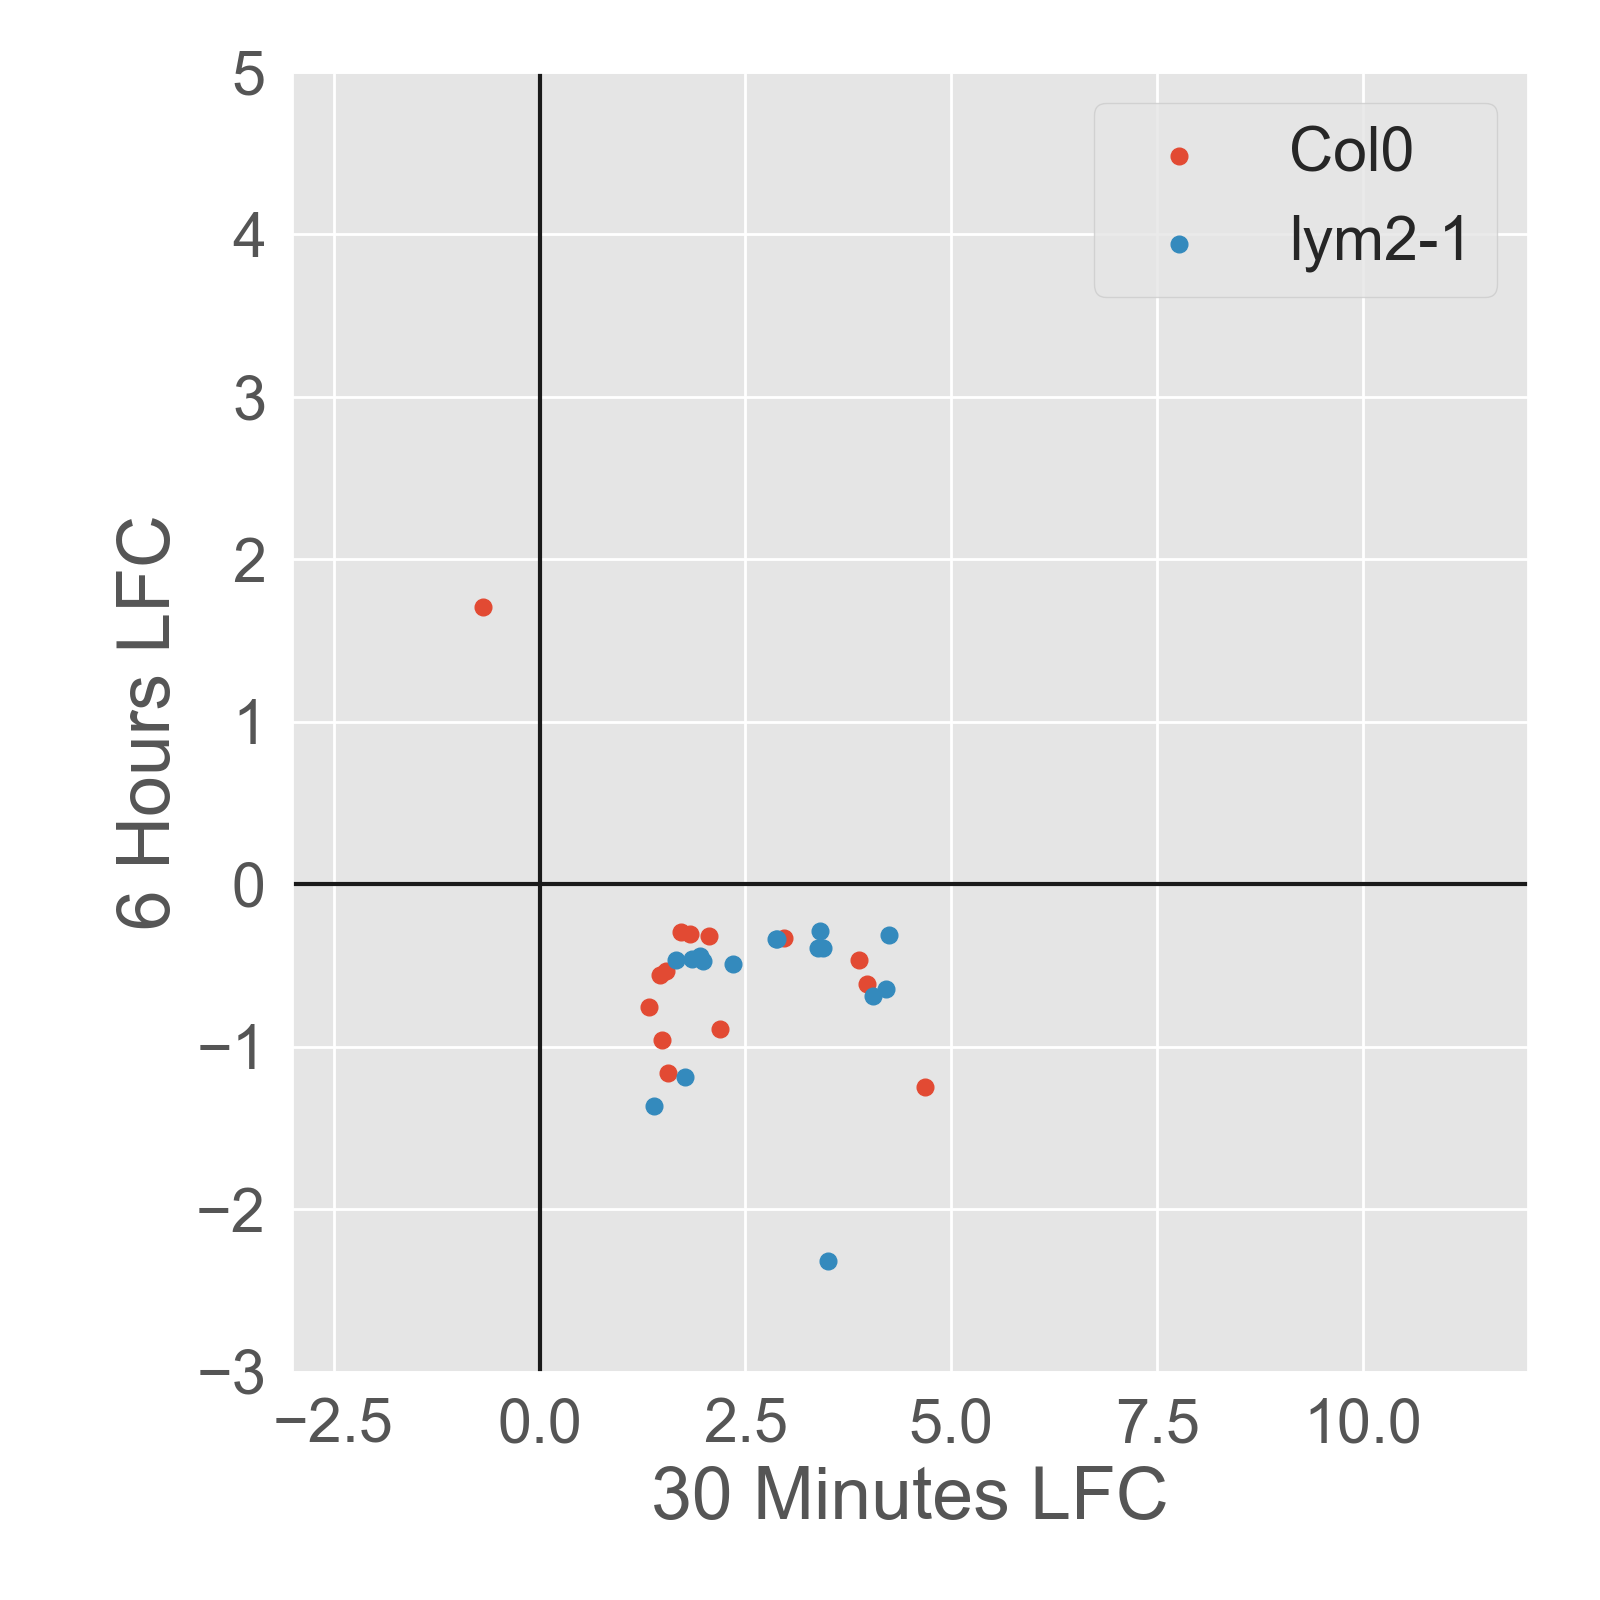
\includegraphics[width=0.5\columnwidth]{./figures/divergingGenes.png}
  }
  \caption{Diverging genes}
  \label{fig:diverg}
\end{figure}



\begin{figure}[!ht]
  \centering
  \subfloat[First sub-figure\label{subfig-2:interest}]{%
    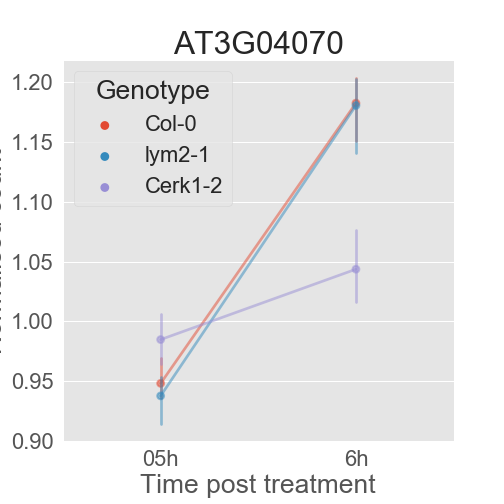
\includegraphics[width=0.7\columnwidth]{./figures/interestingGenes_AT3G04070.png}
  }\\
  \subfloat[First sub-figure\label{subfig-1:interest}]{%
    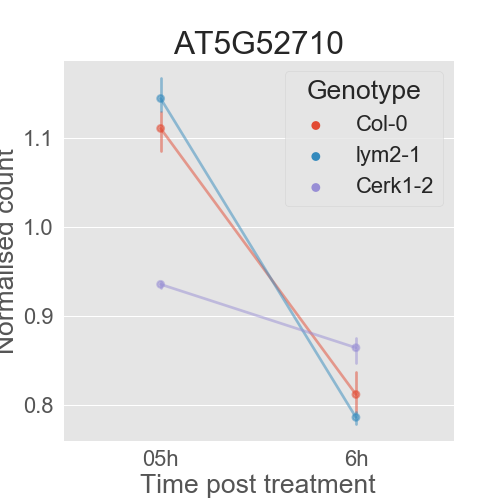
\includegraphics[width=0.7\columnwidth]{./figures/interestingGenes_AT5G52710.png}
  }
  \caption{Interesting genes}
  \label{fig:interestinggenes}
\end{figure}





\section{Analysis of chitin response after 6 hours}
\label{subsec:deg6}
\begin{figure}[ht]
  \centering
  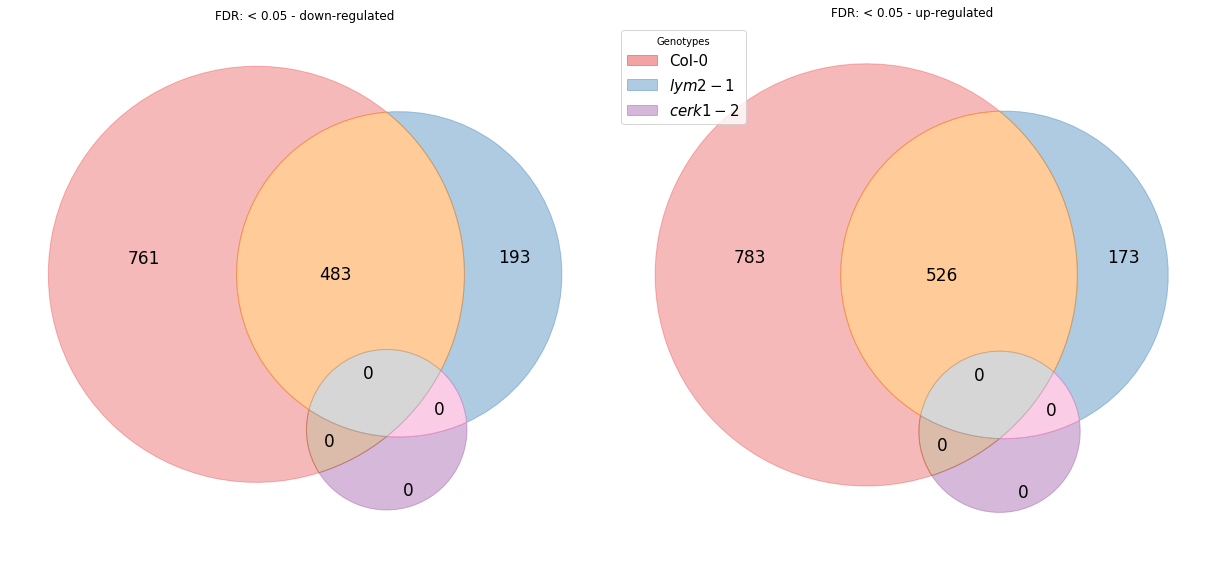
\includegraphics[width=\columnwidth]{figures/vennTreatmentschitin6.png}
  \caption{\label{fig:6hrDEGs} DEGs for 6hr}
\end{figure}



\begin{figure}[!ht]
  \centering
  \subfloat[First sub-figure\label{subfig-1:deg6}]{%
    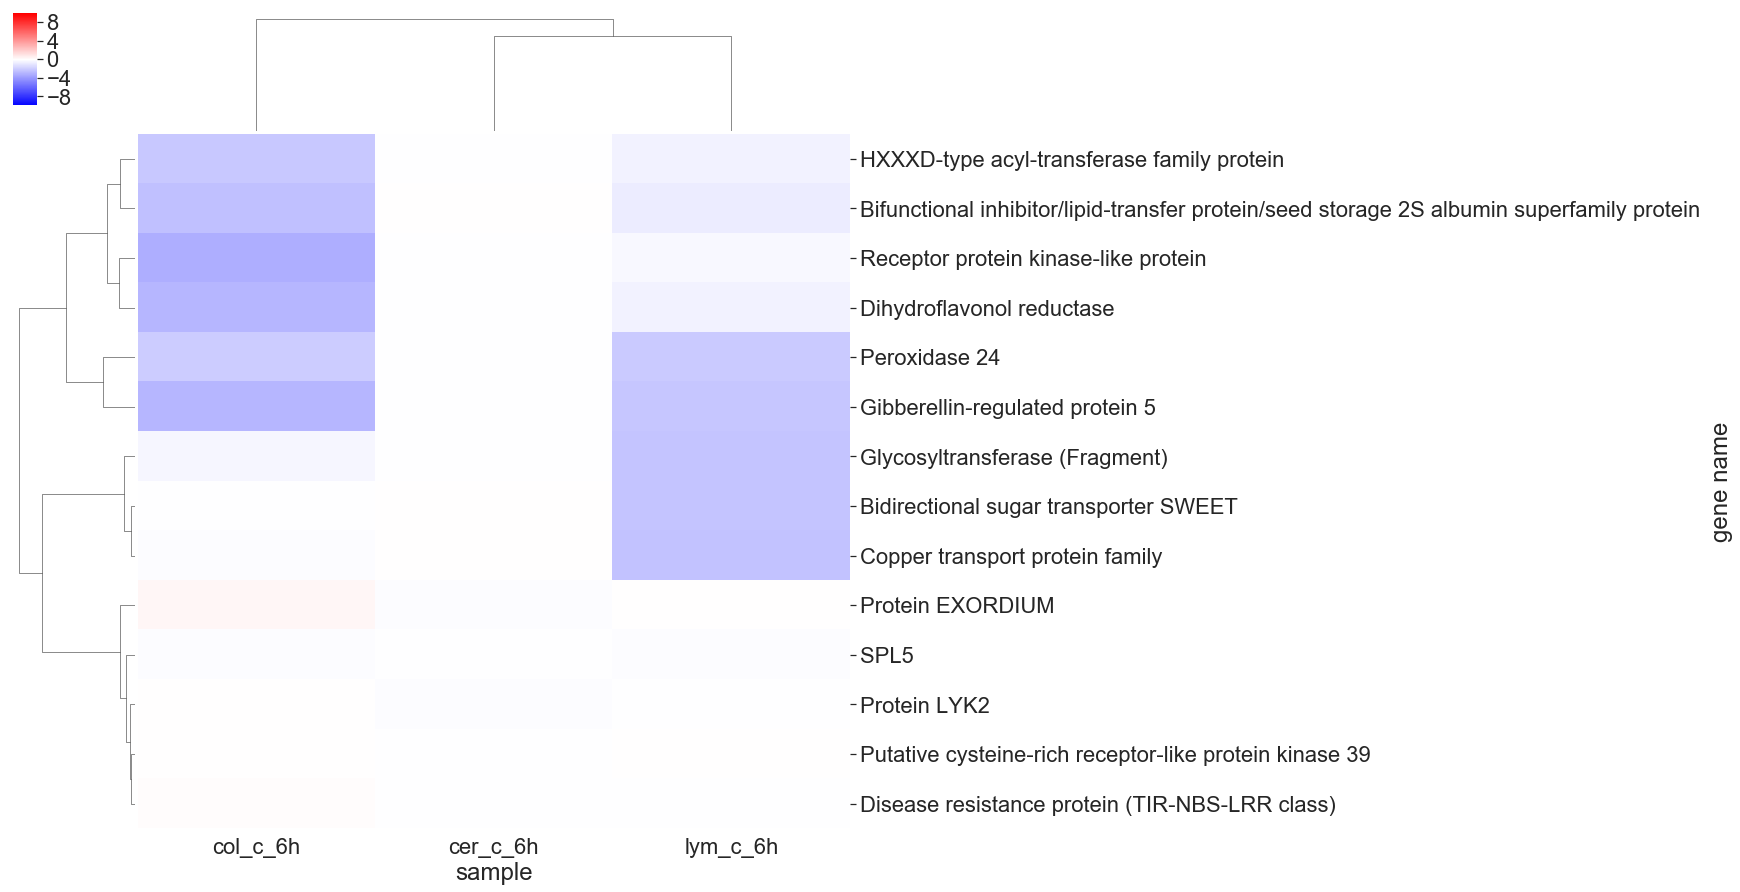
\includegraphics[width=0.7\columnwidth]{./figures/chitin_water_6hr_down.png}
  }
  \\
  \subfloat[First sub-figure\label{subfig-2:deg6}]{%
    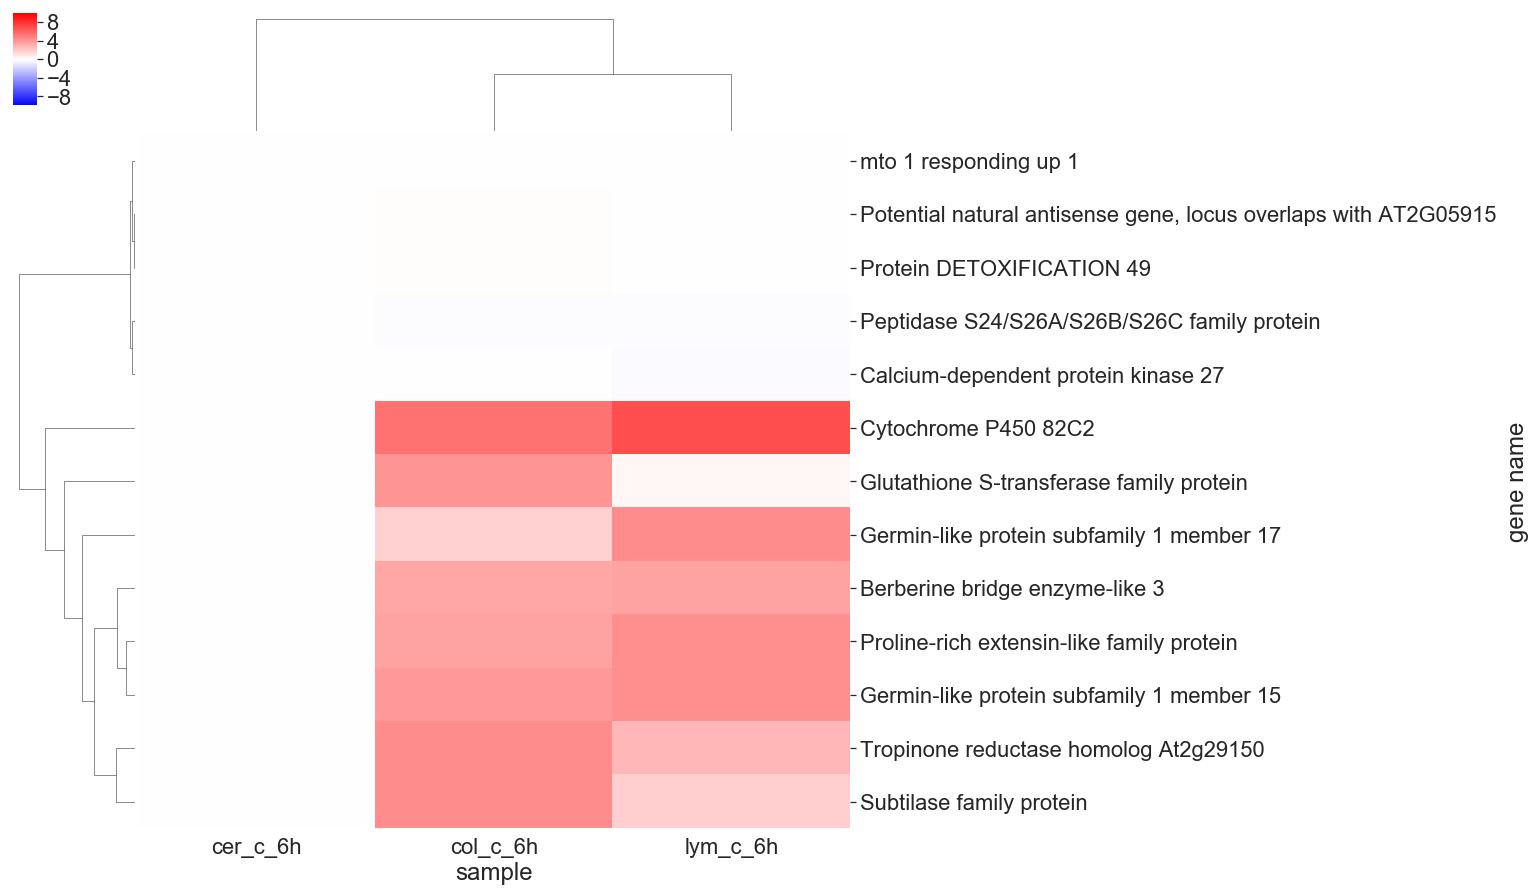
\includegraphics[width=0.7\columnwidth]{./figures/chitin_water_6hr_up.png}
  }
  \caption{DEGs}
  \label{fig:DEG6}
\end{figure}



% trim={5cm 0 0 0},clip




\end{document}


%%% Local Variables:
%%% mode: latex
%%% TeX-master: "../main"
%%% End:
